\documentclass[journal,12pt,twocolumn]{IEEEtran}

\usepackage{setspace}
\usepackage{gensymb}

\singlespacing


\usepackage[cmex10]{amsmath}

\usepackage{amsthm}

\usepackage{mathrsfs}
\usepackage{txfonts}
\usepackage{stfloats}
\usepackage{bm}
\usepackage{cite}
\usepackage{cases}
\usepackage{subfig}

\usepackage{longtable}
\usepackage{multirow}

\usepackage{enumitem}
\usepackage{mathtools}
\usepackage{steinmetz}
\usepackage{tikz}
\usepackage{circuitikz}
\usepackage{verbatim}
\usepackage{tfrupee}
\usepackage[breaklinks=true]{hyperref}
\usepackage{graphicx}
\usepackage{tkz-euclide}
\usepackage{float}

\usetikzlibrary{calc,math}
\usepackage{listings}
    \usepackage{color}                                            %%
    \usepackage{array}                                            %%
    \usepackage{longtable}                                        %%
    \usepackage{calc}                                             %%
    \usepackage{multirow}                                         %%
    \usepackage{hhline}                                           %%
    \usepackage{ifthen}                                           %%
    \usepackage{lscape}     
\usepackage{multicol}
\usepackage{chngcntr}

\DeclareMathOperator*{\Res}{Res}

\renewcommand\thesection{\arabic{section}}
\renewcommand\thesubsection{\thesection.\arabic{subsection}}
\renewcommand\thesubsubsection{\thesubsection.\arabic{subsubsection}}

\renewcommand\thesectiondis{\arabic{section}}
\renewcommand\thesubsectiondis{\thesectiondis.\arabic{subsection}}
\renewcommand\thesubsubsectiondis{\thesubsectiondis.\arabic{subsubsection}}


\hyphenation{op-tical net-works semi-conduc-tor}
\def\inputGnumericTable{}                                 %%

\lstset{
%language=C,
frame=single, 
breaklines=true,
columns=fullflexible
}
\begin{document}
\newtheorem{theorem}{Theorem}[section]
\newtheorem{problem}{Problem}
\newtheorem{proposition}{Proposition}[section]
\newtheorem{lemma}{Lemma}[section]
\newtheorem{corollary}[theorem]{Corollary}
\newtheorem{example}{Example}[section]
\newtheorem{definition}[problem]{Definition}

\newcommand{\BEQA}{\begin{eqnarray}}
\newcommand{\EEQA}{\end{eqnarray}}
\newcommand{\define}{\stackrel{\triangle}{=}}
\bibliographystyle{IEEEtran}
\providecommand{\mbf}{\mathbf}
\providecommand{\pr}[1]{\ensuremath{\Pr\left(#1\right)}}
\providecommand{\qfunc}[1]{\ensuremath{Q\left(#1\right)}}
\providecommand{\sbrak}[1]{\ensuremath{{}\left[#1\right]}}
\providecommand{\lsbrak}[1]{\ensuremath{{}\left[#1\right.}}
\providecommand{\rsbrak}[1]{\ensuremath{{}\left.#1\right]}}
\providecommand{\brak}[1]{\ensuremath{\left(#1\right)}}
\providecommand{\lbrak}[1]{\ensuremath{\left(#1\right.}}
\providecommand{\rbrak}[1]{\ensuremath{\left.#1\right)}}
\providecommand{\cbrak}[1]{\ensuremath{\left\{#1\right\}}}
\providecommand{\lcbrak}[1]{\ensuremath{\left\{#1\right.}}
\providecommand{\rcbrak}[1]{\ensuremath{\left.#1\right\}}}
\theoremstyle{remark}
\newtheorem{rem}{Remark}
\newcommand{\sgn}{\mathop{\mathrm{sgn}}}
\providecommand{\abs}[1]{\vert#1\vert}
\providecommand{\res}[1]{\Res\displaylimits_{#1}} 
\providecommand{\norm}[1]{\lVert#1\rVert}
%\providecommand{\norm}[1]{\lVert#1\rVert}
\providecommand{\mtx}[1]{\mathbf{#1}}
\providecommand{\mean}[1]{E[ #1 ]}
\providecommand{\fourier}{\overset{\mathcal{F}}{ \rightleftharpoons}}
%\providecommand{\hilbert}{\overset{\mathcal{H}}{ \rightleftharpoons}}
\providecommand{\system}{\overset{\mathcal{H}}{ \longleftrightarrow}}
	%\newcommand{\solution}[2]{\textbf{Solution:}{#1}}
\newcommand{\solution}{\noindent \textbf{Solution: }}
\newcommand{\cosec}{\,\text{cosec}\,}
\providecommand{\dec}[2]{\ensuremath{\overset{#1}{\underset{#2}{\gtrless}}}}
\newcommand{\myvec}[1]{\ensuremath{\begin{pmatrix}#1\end{pmatrix}}}
\newcommand{\mydet}[1]{\ensuremath{\begin{vmatrix}#1\end{vmatrix}}}
\numberwithin{equation}{subsection}
\makeatletter
\makeatother
\let\StandardTheFigure\thefigure
\let\vec\mathbf
\renewcommand{\thefigure}{\theproblem}
\def\putbox#1#2#3{\makebox[0in][l]{\makebox[#1][l]{}\raisebox{\baselineskip}[0in][0in]{\raisebox{#2}[0in][0in]{#3}}}}
     \def\rightbox#1{\makebox[0in][r]{#1}}
     \def\centbox#1{\makebox[0in]{#1}}
     \def\topbox#1{\raisebox{-\baselineskip}[0in][0in]{#1}}
     \def\midbox#1{\raisebox{-0.5\baselineskip}[0in][0in]{#1}}
\vspace{3cm}
\title{GATE ASSIGNMENT 2}
\author{Vaibhav Chhabra\\ AI20BTECH11022}
\maketitle
\newpage
\bigskip
\renewcommand{\thefigure}{\theenumi}
\renewcommand{\thetable}{\theenumi}
Download all latex-tikz codes from 
%
\begin{lstlisting}
    https://github.com/vaibhavchhabra25/EE3900-course/blob/main/GATE_Assignment-2/main.tex
\end{lstlisting}
%
Download all python codes from
\begin{lstlisting}
    https://github.com/vaibhavchhabra25/EE3900-course/blob/main/GATE_Assignment-2/codes
\end{lstlisting}

\section{Problem}
(EC 2006-Q.54) The unit-step response of a system starting from rest is given by
\begin{align}
    c(t)=1-e^{-2t} \hspace{0.5cm} \text{for} \  t\geq0 
\end{align}
The transfer function of the system is:
\begin{enumerate}
    \item $\dfrac{1}{1+2s}$ \vspace{0.2cm}
    \item $\dfrac{2}{2+s}$ \vspace{0.2cm}
    \item $\dfrac{1}{2+s}$ \vspace{0.2cm}
    \item $\dfrac{2s}{1+2s}$
\end{enumerate}
\section{Solution}
The input function $r(t)$, to the system is a unit-step function. So, 
\begin{align}
    r(t)=u(t)
\end{align}
The unit-step response for the system is
\begin{align}
    c(t)=1-e^{-2t} \hspace{0.5cm} \text{for} \  t\geq0 
\end{align}
\begin{definition}[Laplace transform]
The Laplace transform of a function f(t) is defined as
\begin{align}
    \mathcal{L}\{f(t)\}(s)=\int_0^\infty f(t)e^{-st}dt
\end{align}
\end{definition}
\begin{definition}[Transfer function]\label{def-2}
The transfer function of a system is defined as the ratio of Laplace transform of the output $c(t)$, to the Laplace transform of the input $r(t)$, under zero initial conditions.
\begin{align}
    T(s)=\dfrac{\mathcal{L}\{c(t)\}(s)}{\mathcal{L}\{r(t)\}(s)}
\end{align}
\end{definition}

The system is given to be starting from rest, so we have zero initial conditions.\\
Now,
\begin{align}
    \mathcal{L}\{c(t)\}(s)=&\mathcal{L}\{1-e^{-2t}\}(s)\\
    =&\int_0^\infty(1-e^{-2t})e^{-st}dt\\
    =&\int_0^\infty e^{-st}dt - \int_0^\infty e^{-(2+s)t}dt\\
    =&\dfrac{1}{s} - \dfrac{1}{2+s}\\
    =&\dfrac{2}{s(2+s)}
\end{align}
And
\begin{align}
    \mathcal{L}\{r(t)\}(s)=&\mathcal{L}\{u(t)\}(s)\\
    =&\mathcal{L}\{1\}(s)\\
    =&\int_0^\infty e^{-st}dt\\
    =&\dfrac{1}{s}
\end{align}
By Definition \ref{def-2},
\begin{align}
    T(s)&=\dfrac{\mathcal{L}\{c(t)\}(s)}{\mathcal{L}\{r(t)\}(s)}\\
    &=\dfrac{\dfrac{2}{s(2+s)}}{\dfrac{1}{s}}\\
    &=\dfrac{2}{2+s}
\end{align}
So, option 2 is correct.

\begin{figure}[!ht]
         \centering
         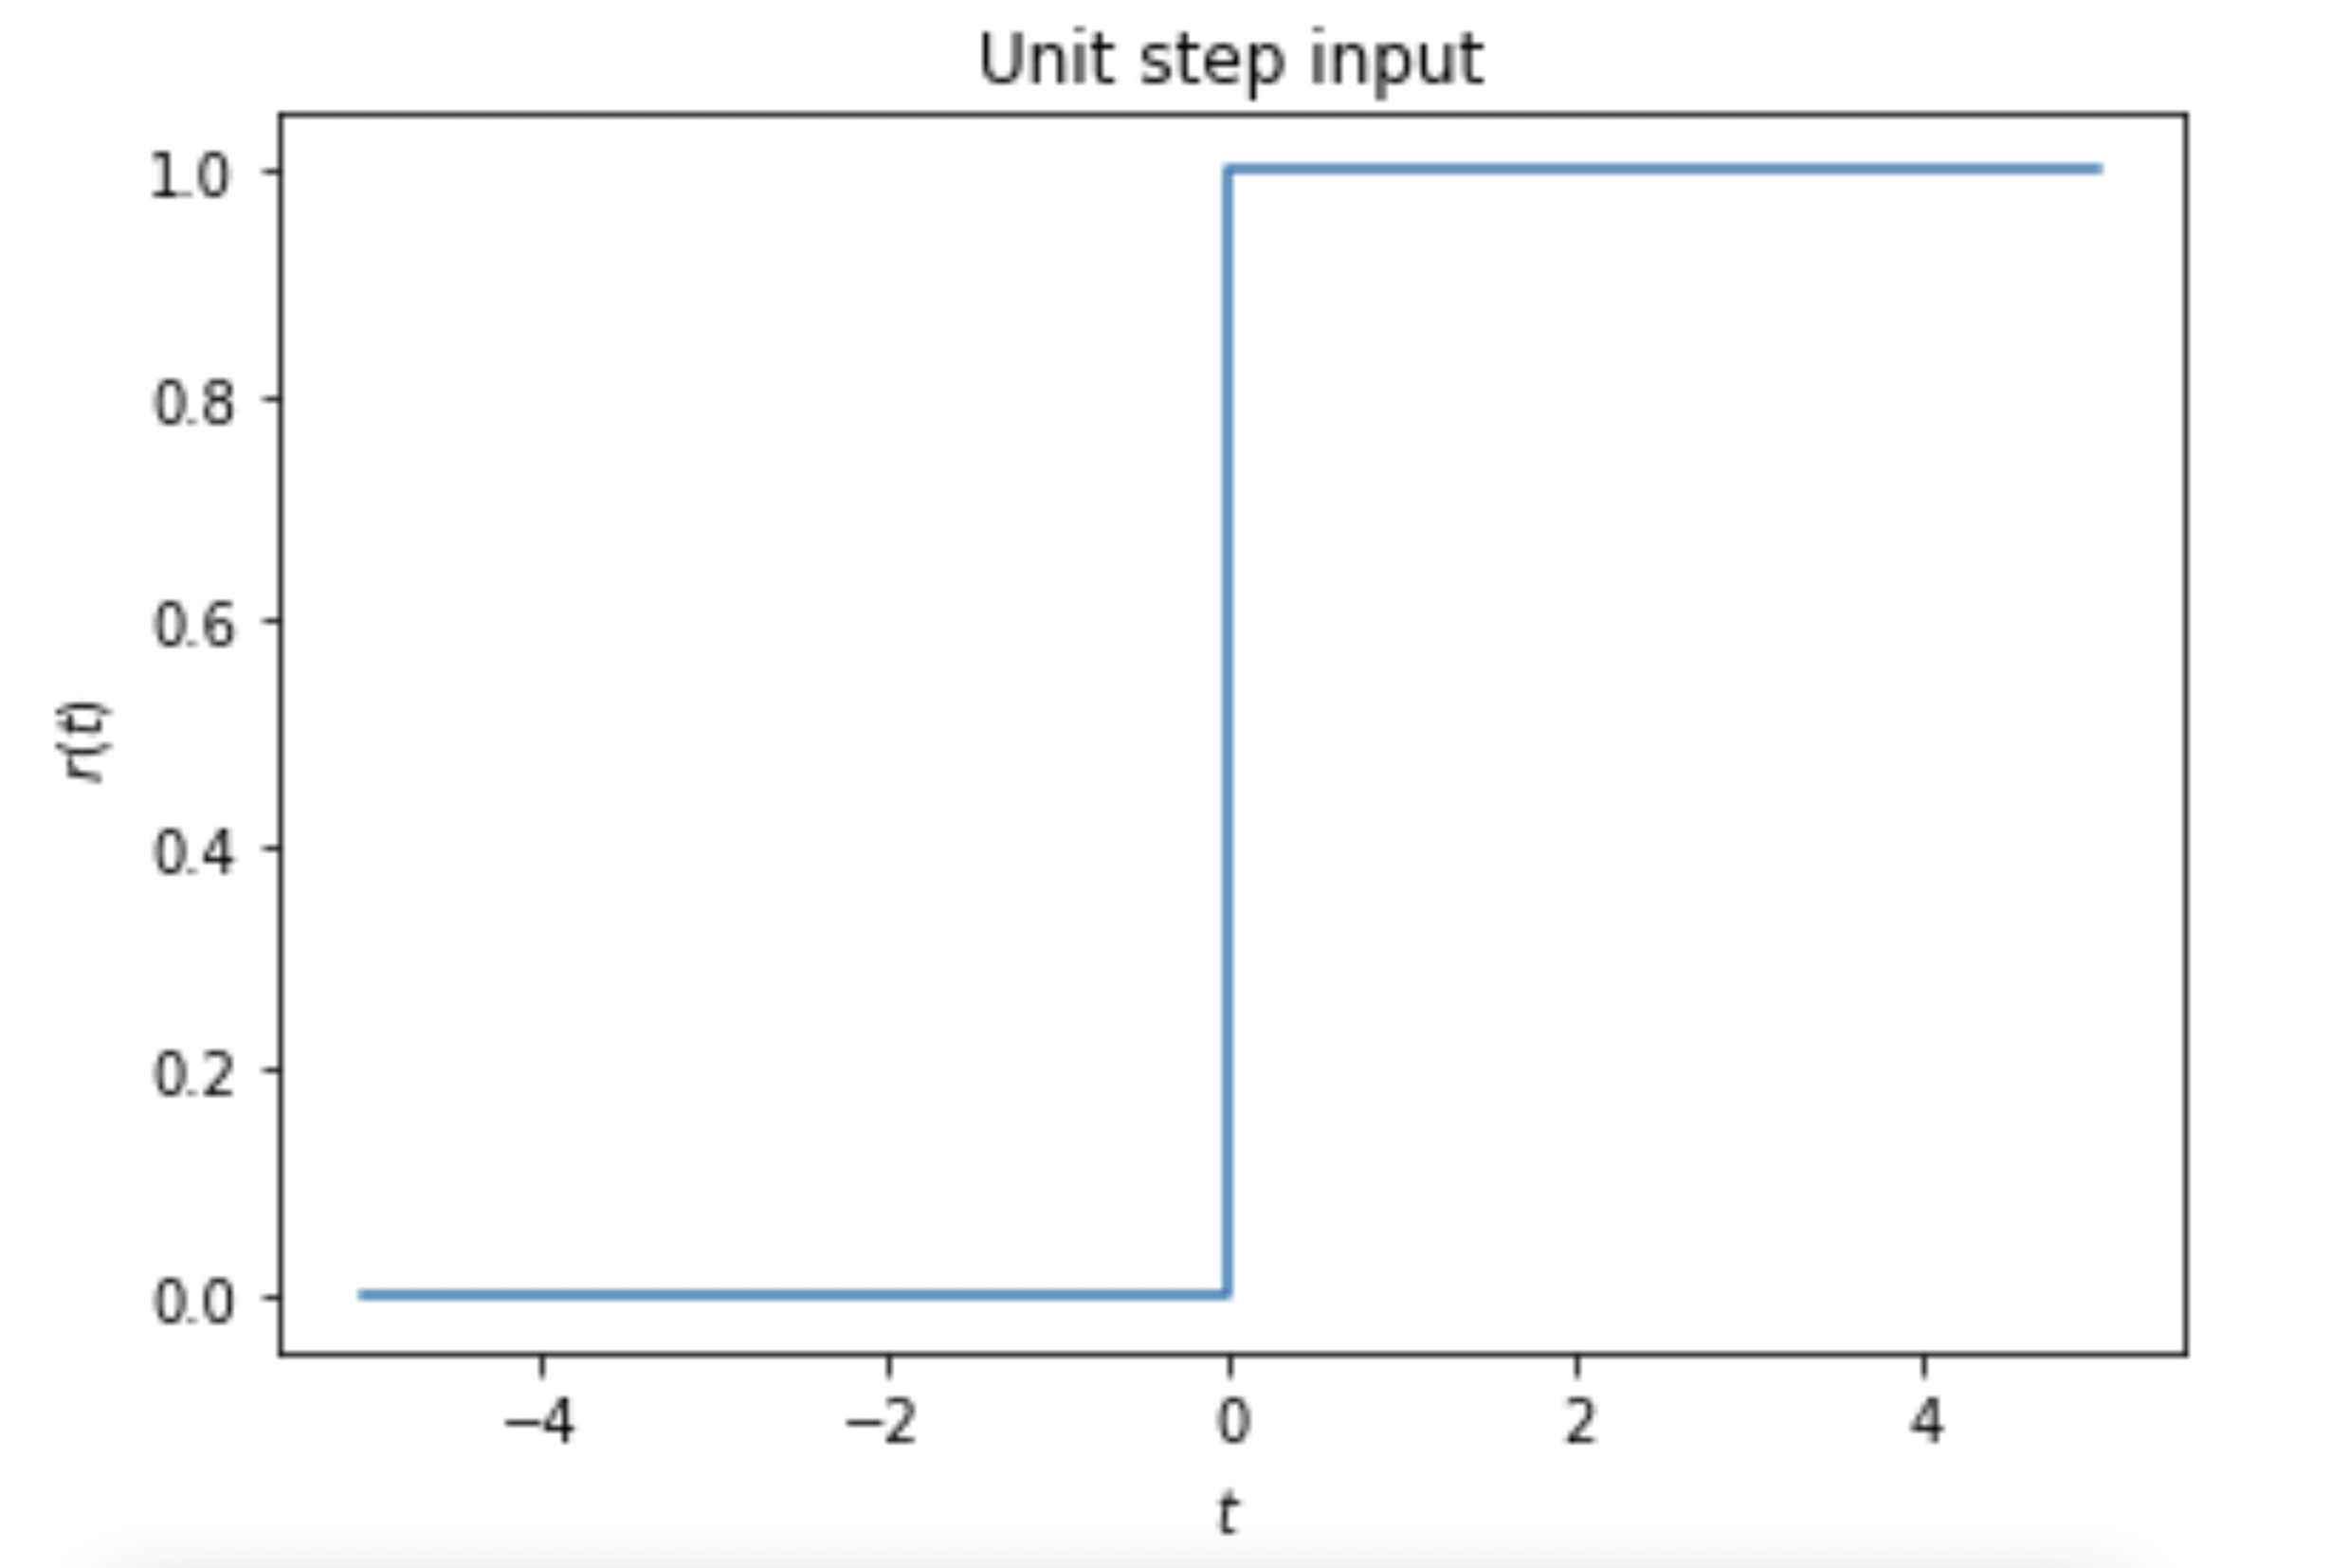
\includegraphics[width=\columnwidth]{input.png}
         \caption{Input Function Plot}
\end{figure}

\begin{figure}[!ht]
         \centering
         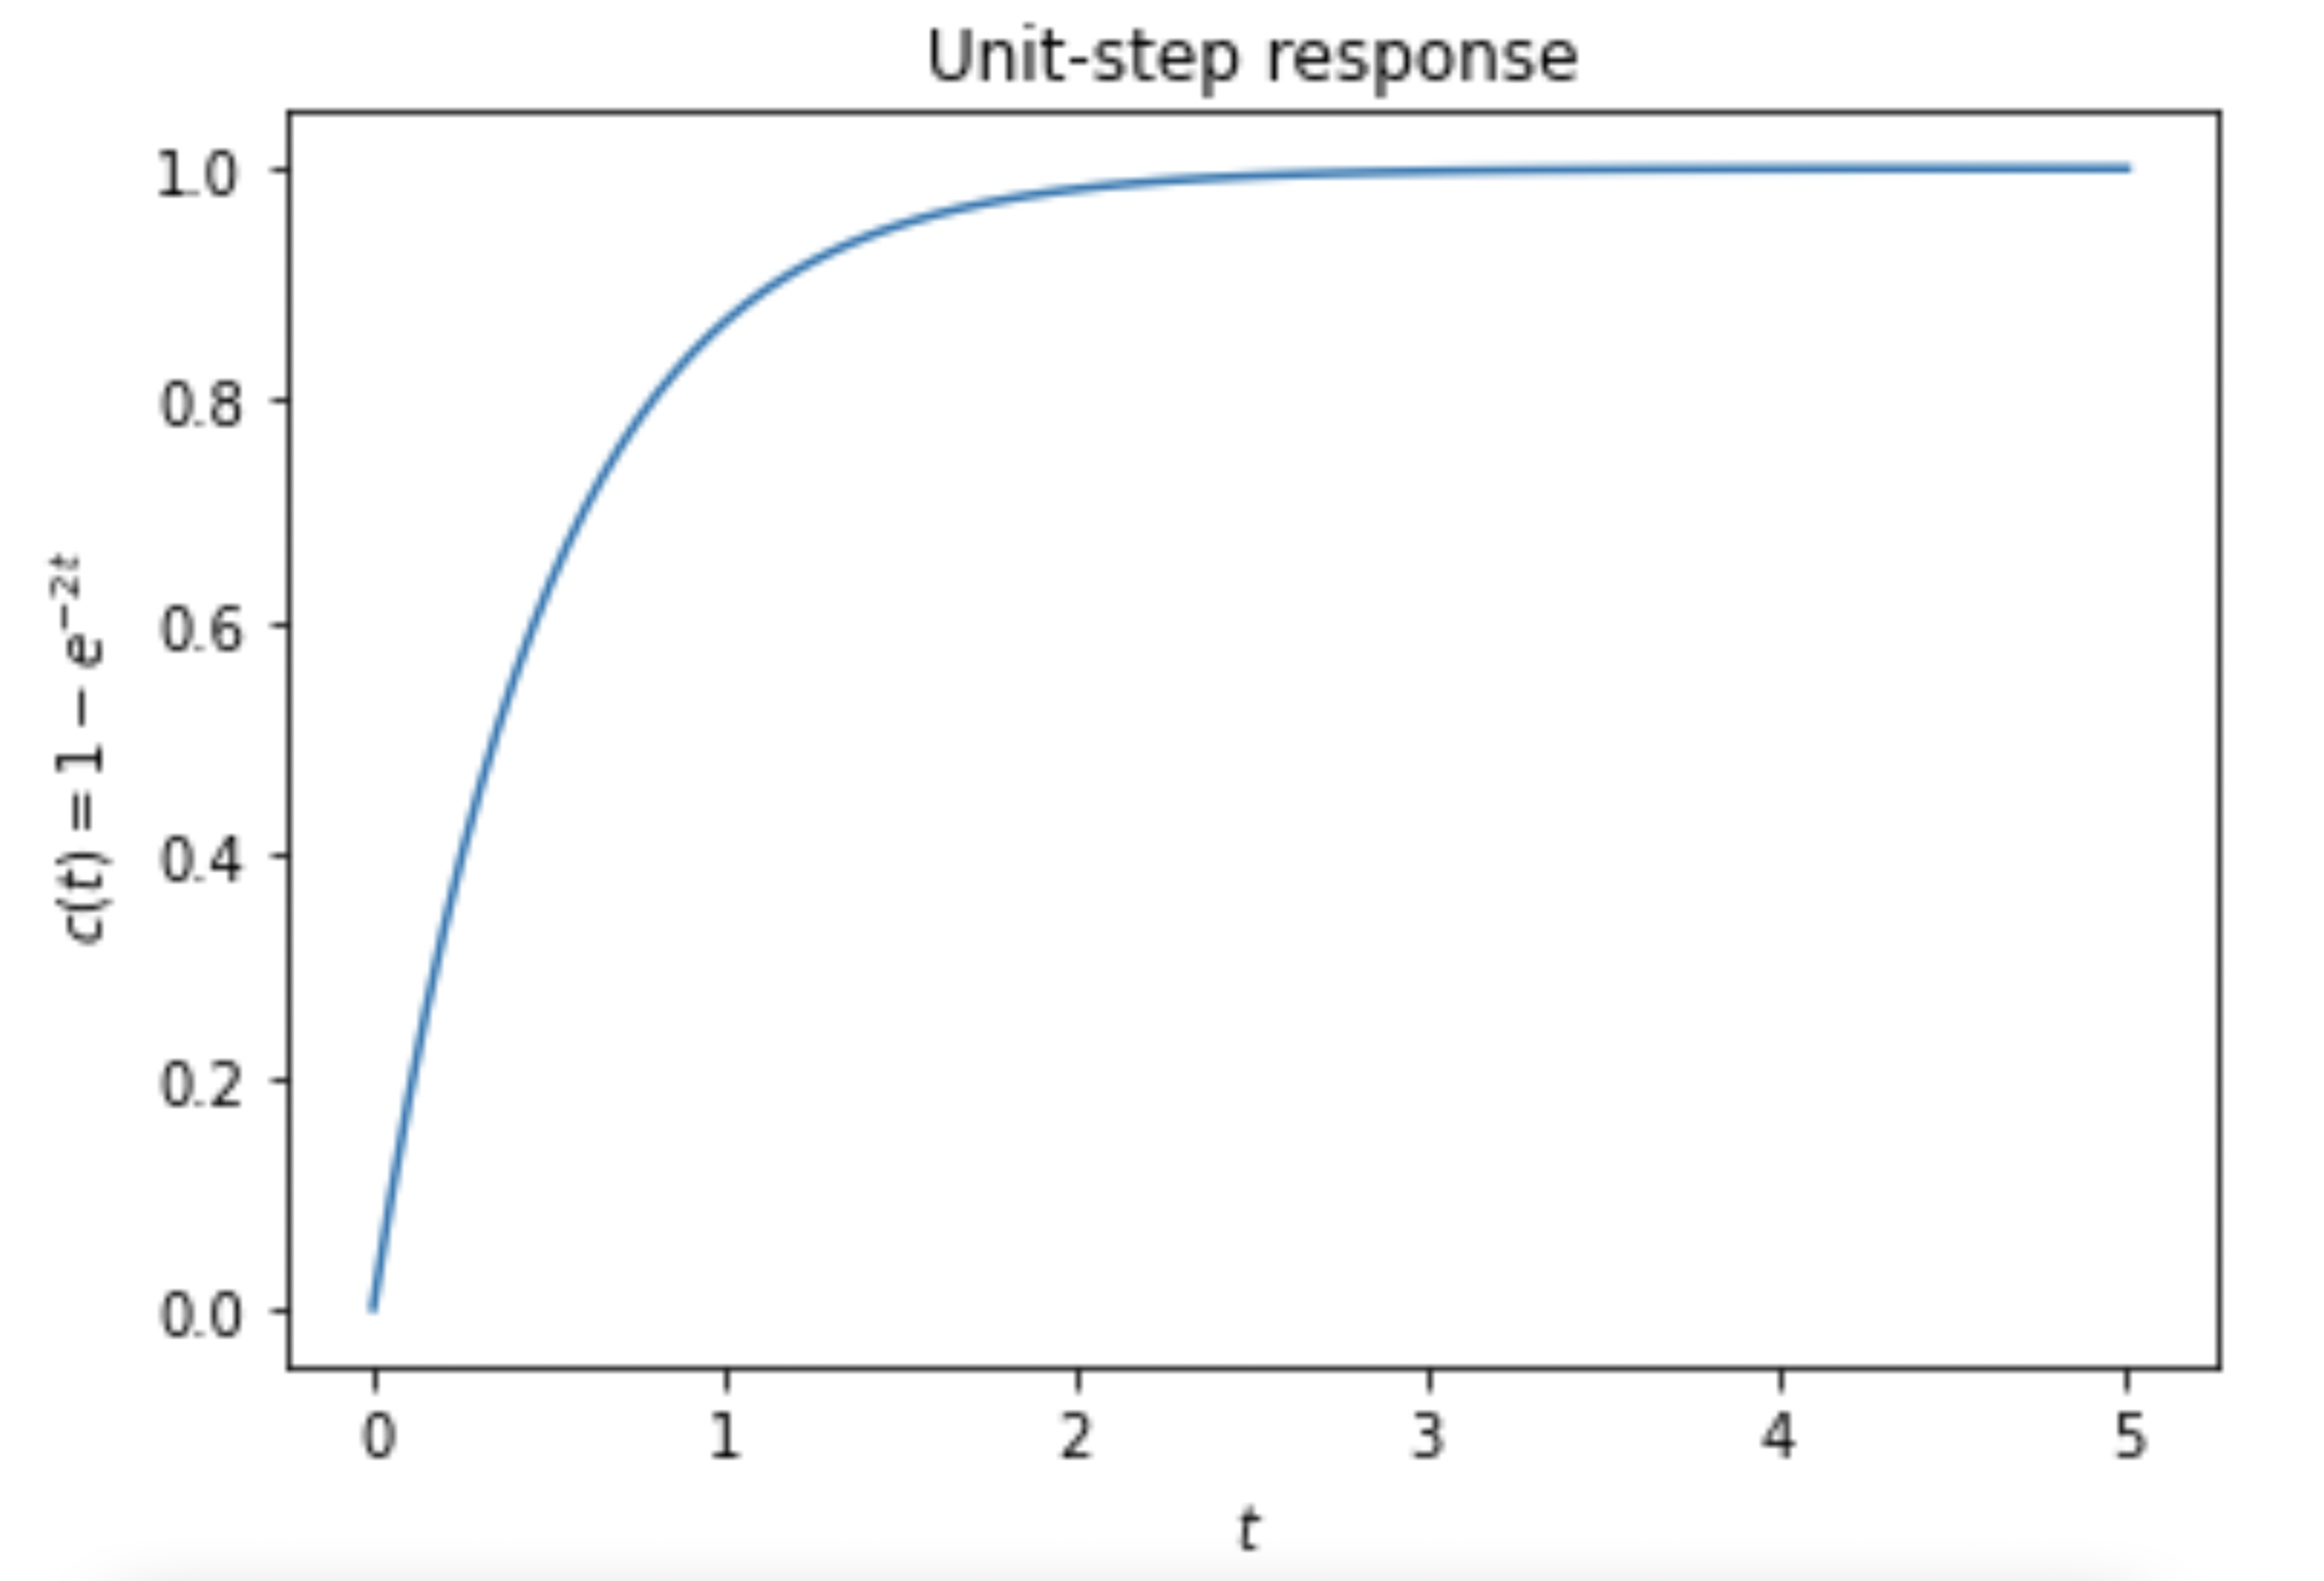
\includegraphics[width=\columnwidth]{response.png}
         \caption{Output Function Plot}
\end{figure}

\begin{figure}[!ht]
         \centering
         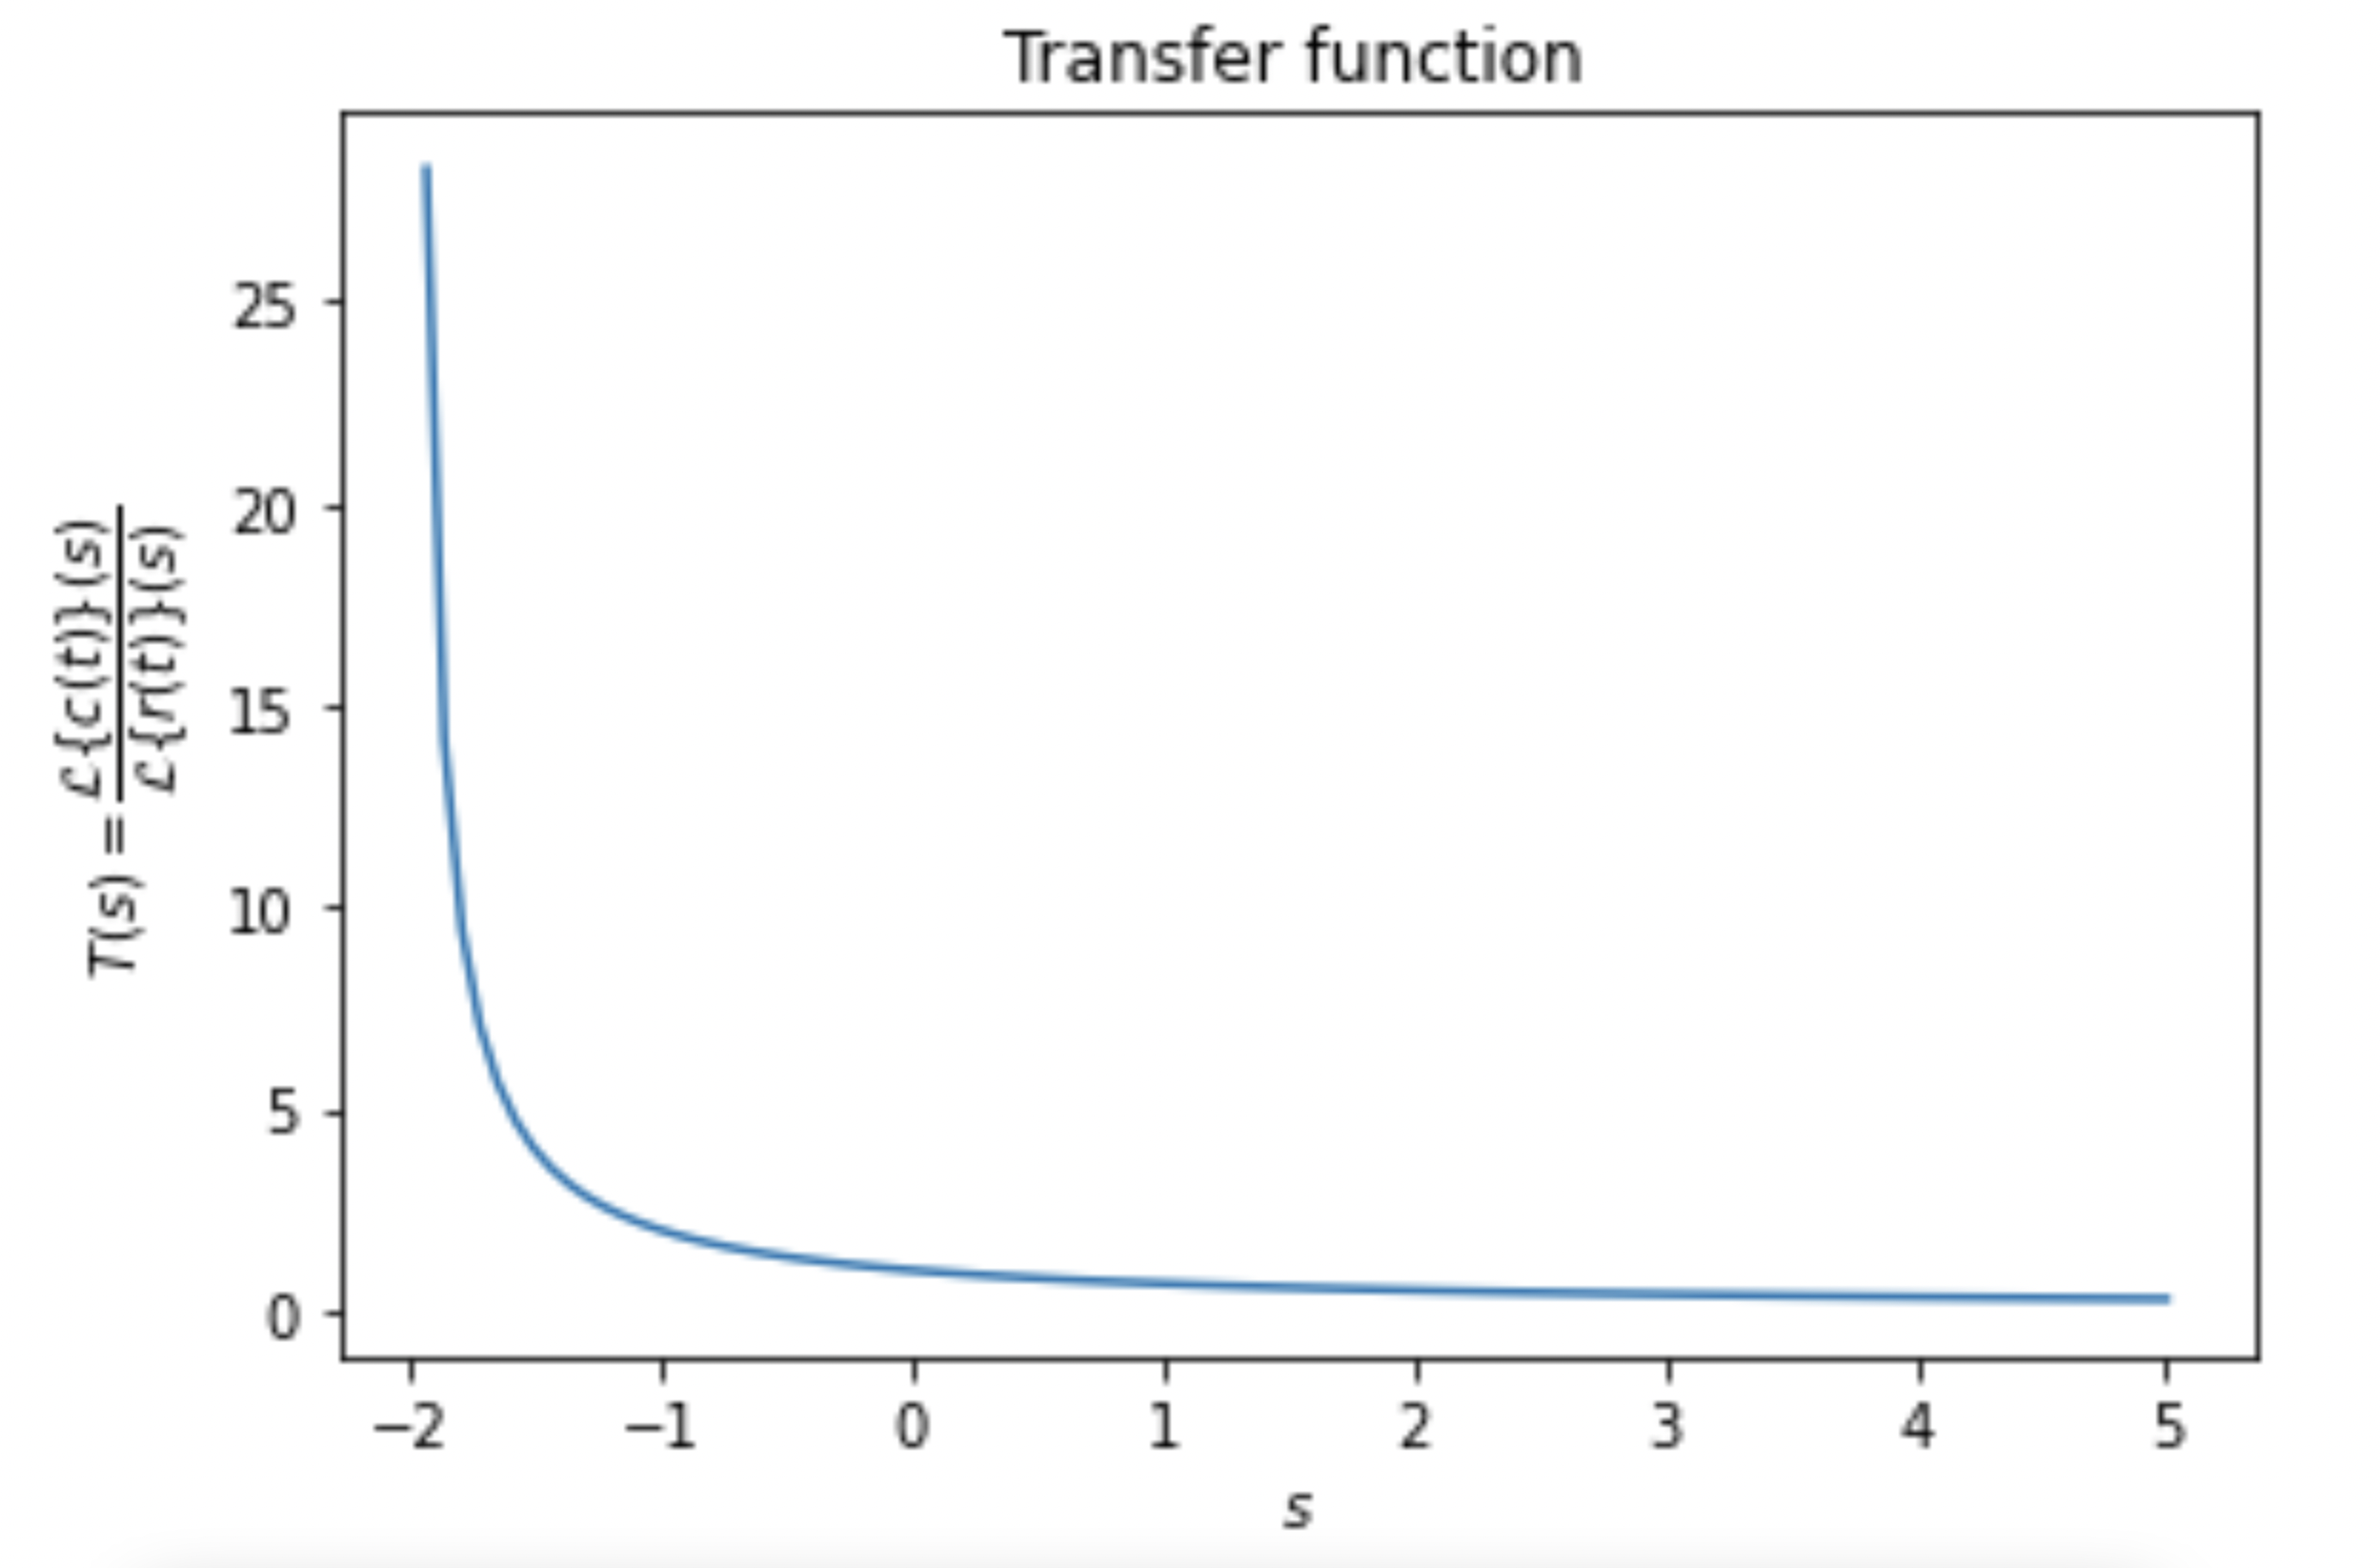
\includegraphics[width=\columnwidth]{TF.png}
         \caption{Transfer Function Plot}
\end{figure}
\end{document}
